\documentclass[fleqn,12pt, a4paper]{article}

\usepackage{psfrag}
\usepackage[dvips]{epsfig}
\usepackage{amsmath,amssymb}
\usepackage{theorem}
\usepackage{epsfig}
\usepackage{color}
\usepackage{mathrsfs}
\usepackage{caption}
\usepackage{graphicx, subfig}

\def\R{{\mathbb R}}
\renewcommand{\Re}{{\mathbb R}}
\def\N{{\mathbb N}}
\def\C{{\mathbb C}}
\def\Z{{\mathbb Z}}
\def\Q{{\mathbb Q}}
\def\C{\mathbb{C}}


\def\I{\mathcal{I}}
\def\A{\mathcal{A}}
\def\B{\mathcal{B}}
\def\U{\mathcal{U}}
\def\V{\mathcal{V}}
\def\W{\mathcal{W}}
\def\F{\mathcal{F}}
\def\Nscr{{\mathcal{N}}}
\def\Mscr{{\mathcal{M}}}

%------------------------------------------------------------
% Theorem like environments
%
\newtheorem{theorem}{Theorem}
\newtheorem{corollary}{Corollary}
\newtheorem{lemma}{Lemma}
\newtheorem{proposition}{Proposition}
%\theoremstyle{plain}
\newtheorem{acknowledgement}{Acknowledgement}
\newtheorem{algorithm}{Algorithm}
\newtheorem{axiom}{Axiom}
\newtheorem{case}{Case}
\newtheorem{claim}{Claim}
\newtheorem{conclusion}{Conclusion}
\newtheorem{condition}{Condition}
\newtheorem{criterion}{Criterion}
\theoremstyle{definition}
\newtheorem{definition}{Definition}
\newtheorem{example}{Example}
\newtheorem{exercise}{Exercise}
\newtheorem{notation}{Notation}
\newtheorem{problem}{Problem}
\newtheorem{remark}{Remark}
\newtheorem{solution}{Solution}
\newtheorem{summary}{Summary}
\numberwithin{equation}{section}
%--------------------------------------------------------

\def\bmat{\left[ \begin{array}}
\def\emat{\end{array} \right]}

\newcommand{\spanop}{\mathop{\rm span}}
\def\bmat{\left[ \begin{array}}
\def\emat{\end{array} \right]}

\headheight 8mm
\headsep 16mm
\topmargin  -20mm
\oddsidemargin -.15in
\textwidth 160mm
\textheight 240mm
\baselineskip 7mm
\parindent 0mm

\def\domain{{\mbox{\em domain}}}
\def\dim{{\mbox{\em dim}}}
\def\range{{\mbox{\sc Range}}}
\def\null{{\mbox{\sc Null}}}
\def\nullity{{\mbox{\sc Nullity}}}
\def\rank{{\mbox{\sc Rank}}}


\def\ifpart{\textbf{(if) }}
\def\onlyifpart{\textbf{(only if) }}
\def\solution{\noindent{\it Solution.} }

\begin{document}
\thispagestyle{plain}

%%%%%%%%%%%%%%%%%%%%%%%%%%%%%%%%%%%%%%%%%%%%%%%%%%%%%%%%%%%%%%%%%%%%%%
\vspace*{-1.5cm}
{\noindent \rule{15.8cm}{.3mm} \\[.3cm]}
\begin{center} \bf
{\large Modeling of the Problem }\medskip
\\
DPOC Programming Excercise \medskip
\\ Nov. 21, 2019. 
\end{center}
\rule{15.8cm}{.3mm} \\[1cm]
%%%%%%%%%%%%%%%%%%%%%%%%%%%%%%%%%%%%%%%%%%%%%%%%%%%%%%%%%%%%%%%%%%%%%%
\section{States, Actions and Disturbance}
\textbf{States}\\
As the system is a time-invariant system, we denote the state space as $S = \{s_1, s_2, \cdots, s_K\}$, $where K = M\times N-num(TREE)$, $s_i = (m_i, n_i, \phi_i)$. There is only one terminal state of the system: $s_T = (m_T, n_T, 1)$, where $map(m_T, n_T) = DROP\_OFF$. At time k, the state is $x_k \in S$.\\

\textbf{Actions}\\
There are five different actions in total, for simplicity, we write actions as $$U=\{(1,0),(-1,0),(0,1),(0,-1),(0,0)\}$$ corresponding to $\{East, West, North, South, Stay\}$ respectively. At time t, the action is $u_k \in U$\\

\textbf{Disturbance}\\
Directly let $\omega_k = x_{k+1}, x_{k+1}\in S$, so the transition matrix is $P_{x_{k+1}|x_k, u_k} = P_{w_k|x_k,u_k}$
\section{State Transition Matrix}
The State Transition can be divided into 4 substeps: take action, moved by wind, shoot by the resident and pick up. In order to figure out the exact transition of each substep, we introduce 3 internal states $x_k^1, x_k^2, x_k^3$, which denote the state of the drone after taking 1-3 substeps, as is illustrated in Figure 1.\\

\begin{figure}[htp]
\centering  
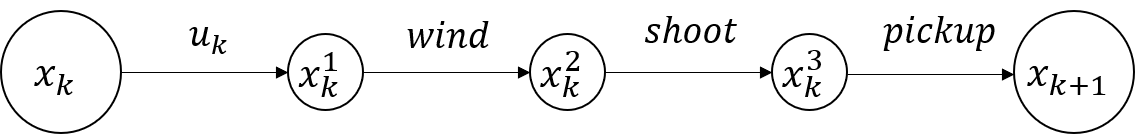
\includegraphics[width=0.6\textwidth]{substates.png}
\caption{Substeps in one stage}
\label{substep}
\end{figure}

Consider the influence of crash or teminal directly on the next states disregarding the internal states (e.g. if $x_k^2$ crash then  $x_{k+1}$ can only be in base; if $x_k$ is terminal states, then $x_{k+1}$ can only be in ternimal states), we introduce extra states $C$ and $T$ for internal statespace. $C$ means already crash and $T$ means $x_k$ already in terminal in the last stage. Therefore, we have:
\begin{align*}
&x_k \in S\\
 &x_k^1 \in S\cup\{T\}\\
 &x_k^2 \in S\cup\{C\}\cup\{T\}\\
 &x_k^3 \in S\cup\{C\}\cup\{T\}\\
 &x_{k+1} \in S
\end{align*}
In this way, the transition probability canbe calculated as:
\begin{align*}
P(x_{k+1}|x_k,u_k) = P(x_k^1|x_k,u_k)P(x_k^2|x_k^1)P(x_k^3|x_k^2)P(x_{k+1}|x_k^3)
\end{align*}
In the following subsections, we will discuss each part in order.


\subsection{Substage 1}
In this substage we will calculate $P(x_k^1|x_k,u_k)$, $x_k^1$ means the state after taking the action, without wind and shoot. We consider the after taking the action that is not allowed, i.e. will arrive at tree or out of bound, we set the state to stay. In the stage cost section, we set the cost of unallowable action to be larger than cost of stay, so it will not be considered in the optimizing process. It can be written as:

\begin{align*}
&P(x_k^1|x_k\in S/s_T,u_k)=
0,\quad if\quad crash \\
&P(x_k^1|x_k\in S/s_T,u_k)=
\begin{cases}
1, \quad x_k^1=x_k+u_k\\
0, \quad x_k^1=otherstates\\
\end{cases}\\
&P(x_k^1|x_k=s_T, u_k)=
\begin{cases}
1, \quad x_k^1 = T \\
0, \quad x_k^1=otherstates\\
\end{cases}
\end{align*}




\subsection{Substage 2}
In this substate we will calculate $P(x_k^2|x_k^1)$, $x_k^2$ means the state after taking the action, after moved by the wind, not been shot yet. It can be written as:
\begin{align*}
&P(x_k^2|x_k^1\in S)=
\begin{cases}
\frac{p_{wind}}{4}, \quad x_k^2=crash? C:x_k^1+(1,0,0)^T\\
\frac{p_{wind}}{4}, \quad x_k^2=crash? C:x_k^1+(0,1,0)^T\\
\frac{p_{wind}}{4}, \quad x_k^2=crash? C:x_k^1+(-1,0,0)^T\\
\frac{p_{wind}}{4}, \quad x_k^2=crash? C:x_k^1+(0,-1,0)^T\\
1-p_{wind}, \quad x_k^2=x_k^1
0, \quad x_k^2=otherstates
\end{cases}\\
&P(x_k^2|x_k^1=T)=
\begin{cases}
1, \quad x_k^2=T\\
0, \quad x_k^2=otherstates
\end{cases}\\
\end{align*}

\subsection{Substage 3}
In this substate we will calculate $P(x_k^3|x_k^2)$, $x_k^3$ means the state after taking the action, after moved by the wind, and after being shot. It can be written as:
\begin{align*}
&P(x_k^3|x_k^2\in shotrange)=
\begin{cases}
\prod_{i=0}^{m}(1-\frac{\gamma}{d_i+1}), \quad x_k^3=x_k^2\\
1-\prod_{i=0}^{m}(1-\frac{\gamma}{d_i+1}), \quad x_k^3 =C \\
0, \quad x_k^3 = otherstates
\end{cases}\\
&P(x_k^3|x_k^2\in S/shotrange)=
\begin{cases}
1, \quad x_k^3=x_k^2\\
0, \quad x_k^3=otherstates
\end{cases}\\
&P(x_k^3|x_k^2=C)=
\begin{cases}
1, \quad x_k^3=C\\
0, \quad x_k^3=otherstates
\end{cases}\\
&P(x_k^3|x_k^2=T)=
\begin{cases}
1, \quad x_k^3=T\\
0, \quad x_k^3=otherstates
\end{cases}\\
\end{align*}

\subsection{Substage 4}
In this substate we will calculate $P(x_{k+1}|x_k^3)$. We denote the special state to change $\phi$ as pickupstate, which is $(m_p,n_p,0)$. The transition matrix can be written as:
\begin{align*}
&P(x_{k+1}|x_k^3\in S/pickupstate)=
\begin{cases}
1, \quad x_{k+1}=x_k^3\\
0, \quad x_{k+1}=otherstates
\end{cases}\\
&P(x_{k+1}|x_k^3=pickupstate)=
\begin{cases}
1, \quad x_{k+1}=x_k^3+(0,0,1)^T\\
0, \quad x_{k+1}=otherstates
\end{cases}\\
&P(x_{k+1}|x_k^3=C)=
\begin{cases}
1, \quad x_{k+1}=basestate\\
0, \quad x_{k+1}=otherstates
\end{cases}\\
&P(x_{k+1}|x_k^3=T)=
\begin{cases}
1, \quad x_{k+1}=s_T\\
0, \quad x_{k+1}=otherstates
\end{cases}\\
\end{align*}


\section{State Cost}
We can use dynamic programming method to evaluate the cost in each stage by backpropagating among substates.
Because the stage cost is irrelavant to the state $x_{k+1}$, given $x_k^3$. So we directly update cost from $x_k^3$:
\begin{align*}
g_3(x_k^3) = 
\begin{cases}
N_c, \quad x_k^3=C\\
0, \quad x_k^3=T\\
1, \quad x_k^3=otherstates
\end{cases}
\end{align*}
Then $g_2(x_k^2$ and $g_1(x_k^1)$ can be updtated in order:
\begin{align*}
&g_2(x_k^2) = p(x_k^3|x_k^2)g_3(x_k^3)\\
&g_1(x_k^1) = p(x_k^2|x_k^1)g_2(x_k^3)
\end{align*}
Finally, $g_k(x_k,u_k)$ can be computed considering the not allowed action:
\begin{align*}
&g_k(x_k, u_k) = 
\begin{cases}
inf+p(x_k^1|x_k,u_k)g_1(x_k^1), \quad x_k+u_k\rightarrow crashed\\
p(x_k^1|x_k,u_k)g_1(x_k^1), \quad otheractions\\
\end{cases}
\end{align*}




\end{document}